\documentclass{standalone}
\usepackage{tikz}
\usepackage{pgfplots}
\usetikzlibrary{arrows.meta}

\begin{document}

\resizebox{8cm}{8cm}{%
    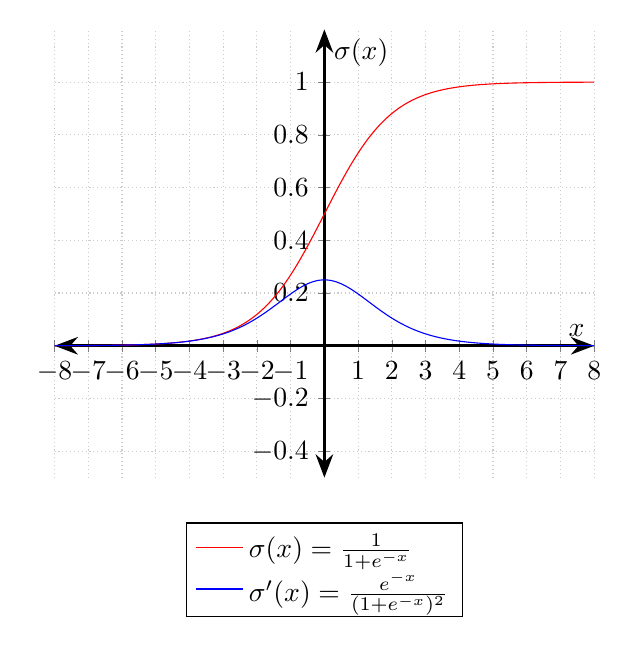
\begin{tikzpicture}
    \begin{axis}[
        title={},
        axis lines=middle,
        axis line style={Stealth-Stealth,very thick},
        xlabel=$x$,
        ylabel={$\sigma(x)$},
        xmin=-8,xmax=8,ymin=-0.5,ymax=1.2,
        xtick distance=1,
        ytick distance=1,
        grid=major,
        grid style={thin,densely dotted,black!20},
        % Numbers on axes
        xtick={-8,-7,-6,-5,-4,-3,-2,-1,0,1,2,3,4,5,6,7,8},
        ytick={-0.4,-0.2,0,.2,.4,.6,.8,1},
        % Legend
        legend style={
            at={(0.5,-0.1)}, % Position at the center bottom
            anchor=north, % Anchor the legend at the top
            cells={anchor=west} % Align the legend entries to the left
        }
    ]
    % Plot the sigmoid function
    \addplot[
        domain= -8:8,
        samples=200,
        color=red
        ]
        {1/(1 + exp(-x))};

    % Plot the dirivative of the sigmoid function
    \addplot[
        domain= -8:8,
        samples=200,
        color=blue
        ]
        {exp(-x)/(1 + exp(-x))^2};
    \addlegendentry{$\sigma(x) = \frac{1}{1 + e^{-x}}$}
    \addlegendentry{$\sigma'(x) = \frac{e^{-x}}{(1 + e^{-x})^2}$}
    \end{axis}
    \end{tikzpicture}
}

\end{document}